%File Generated with PyPaper
\documentclass[aps,prl,amsmath,amssymb,superscriptaddress,notitlepage,groupedaddress]{revtex4-1}
\usepackage{graphicx}
\usepackage{dcolumn}
\usepackage{stackengine}
\usepackage[section]{placeins}
\usepackage[dvipsnames*,svgnames]{xcolor}
\usepackage{verbatim}
\usepackage[position=bottom,caption=false,captionskip=3pt,font=normalsize,subrefformat=simple,labelformat=simple]{subfig}
\renewcommand{\thesubfigure}{(\alph{subfigure})}
\usepackage{listings}
\usepackage{mathtools}
\usepackage{todonotes}
\usepackage{amsmath}
\usepackage{chngcntr}
\usepackage{bm}
\usepackage{url}
\def\UrlBreaks{\do\/\do-}
\newcommand {\framedgraphic}[2] {\begin{frame}{#1}\begin{center}\includegraphics[width=\textwidth,height=0.8\textheight,keepaspectratio]{#2}\end{center}\end{frame}}\usepackage[breaklinks]{hyperref}
\usepackage{tabularx}
\usepackage{soul}
\hypersetup{
colorlinks,
linkcolor={blue!100!black},
citecolor={blue},
urlcolor={blue!80!black}}
\lstset{basicstyle=\small\ttfamily,columns=flexible,breaklines=true}\newcommand{\fakesection}[1]{\par\refstepcounter{section}\sectionmark{#1}\addcontentsline{toc}{section}{\protect\numberline{\thesection}#1}}\def\equationautorefname~#1\null{#1\null}
\raggedbottom\usepackage[bottom]{footmisc} \makeatletter \def\p@section{} \def\p@subsubsection{} \makeatother\begin{document}
\title{\texttt{bayesim}: a tool for fast model fitting with Bayesian inference}
\author{Rachel Kurchin}
\affiliation{Department of Materials Science \& Engineering, Massachusetts Institute of Technology, 77 Massachusetts Avenue, Cambridge, MA 02139, USA}
\author{Giuseppe Romano}
\affiliation{Department of Mechanical Engineering, Massachusetts Institute of Technology, 77 Massachusetts Avenue, Cambridge, MA 02139, USA}
\author{Tonio Buonassisi}
\email{buonassi@mit.edu}
\affiliation{Department of Mechanical Engineering, Massachusetts Institute of Technology, 77 Massachusetts Avenue, Cambridge, MA 02139, USA}

\begin{abstract}
Target journal: Computer Physics Communications
\end{abstract}

\maketitle

\section*{Introduction}
  There are a plethora of examples across diverse scientific and engineering fields of mathematical models used to simulate the results of experimental observations. In many cases, there are input parameters to these models which are difficult to determine via direct measurement, and it is desirable to invert the numerical model -- that is, use the experimental observations to determine values of the input parameters. Bayesian inference is a fruitful framework within which to do such fitting, since the resulting posterior probability distribution over the parameters of interest can give rich insights into not just the most likely values of the parameters, but also uncertainty about these values and the potentially complicated ways in which they can covary to give equally good fits to observations.

  We have previously demonstrated the value of a Bayesian approach in using automated high-throughput temperature- and illumination-dependent current-voltage measurements (JVTi) to fit material/interface properties and defect recombination parameters in photovoltaic (PV) absorbers~\cite{SnSJoule,FeBayes}. In cases such as these, when the data model is not a simple analytical equation but rather a computationally intensive numerical model, efficient, nonredundant sampling of the parameter space when computing likelihoods becomes critical to making the fit feasible.

  In this work, we introduce \texttt{bayesim}, a Python-based code that utilizes adaptive grid sampling to perform Bayesian parameter estimation. We discuss the structure of the code, its implementation, and provide several examples of its usage. While the authors' expertise is in the realm of semiconductor physics and thus the examples herein are drawn from that space, we also discuss the general characteristics of a problem amenable to this approach so that researchers from other fields might adopt it as well.

\section*{Technical Background}

 Bayes' Theorem is a relationship between conditional probabilities. It states

 \begin{equation}
   \begin{split}
     \label{Eq:1001}
     P(H|E)=\frac{P(H)P(E|H)}{P(E)}
   \end{split}
 \end{equation}

 where the notation $P(A|B)$ indicates the probability of $A$ being true given that $B$ is true. $H$ is a \textit{hypothesis} and $E$ the observed \textit{evidence}. $P(H)$ is termed the \textit{prior}, $P(E|H)$ the \textit{likelihood}, $P(H|E)$ the \textit{posterior}, and $P(E)$ is a normalizing constant. If there are $n$ pieces of evidence, this can generalize to an iterative process where

 \begin{equation}
   \begin{split}
     \label{Eq:2}
     P(H|\{E_1,E_2,...E_n\}) = \frac{P(H|\{E_1,E_2...E_{n-1}\})P(E_n|H)}{P(E_n)}
   \end{split}
 \end{equation}

 In a multidimensional parameter estimation problem, each hypothesis $H$ is a tuple of possible values for the fitting parameters, i.e. a point in the parameter space, while the evidence $E$ is an observed output of a measurement as a function of various experimental conditions.

 In order to compute a likelihood, a model capable of simulating that observed output as a function of both the fitting parameters and the experimental conditions is required. In \texttt{bayesim}, likelihoods are calculated for each point in parameter space using a Gaussian where the argument is the difference between observed and simulated output at that point, and the standard deviation is the sum of experimental uncertainty and model uncertainty. The experimental uncertainty is a number provided by the user that quantifies any noise/irreproducibility inherent to the measurement, while the model uncertainty is calculated by \texttt{bayesim} and reflects the sparseness of the parameter space grid, i.e. how much simulated output changes from one grid point to another.

 \begin{figure}
   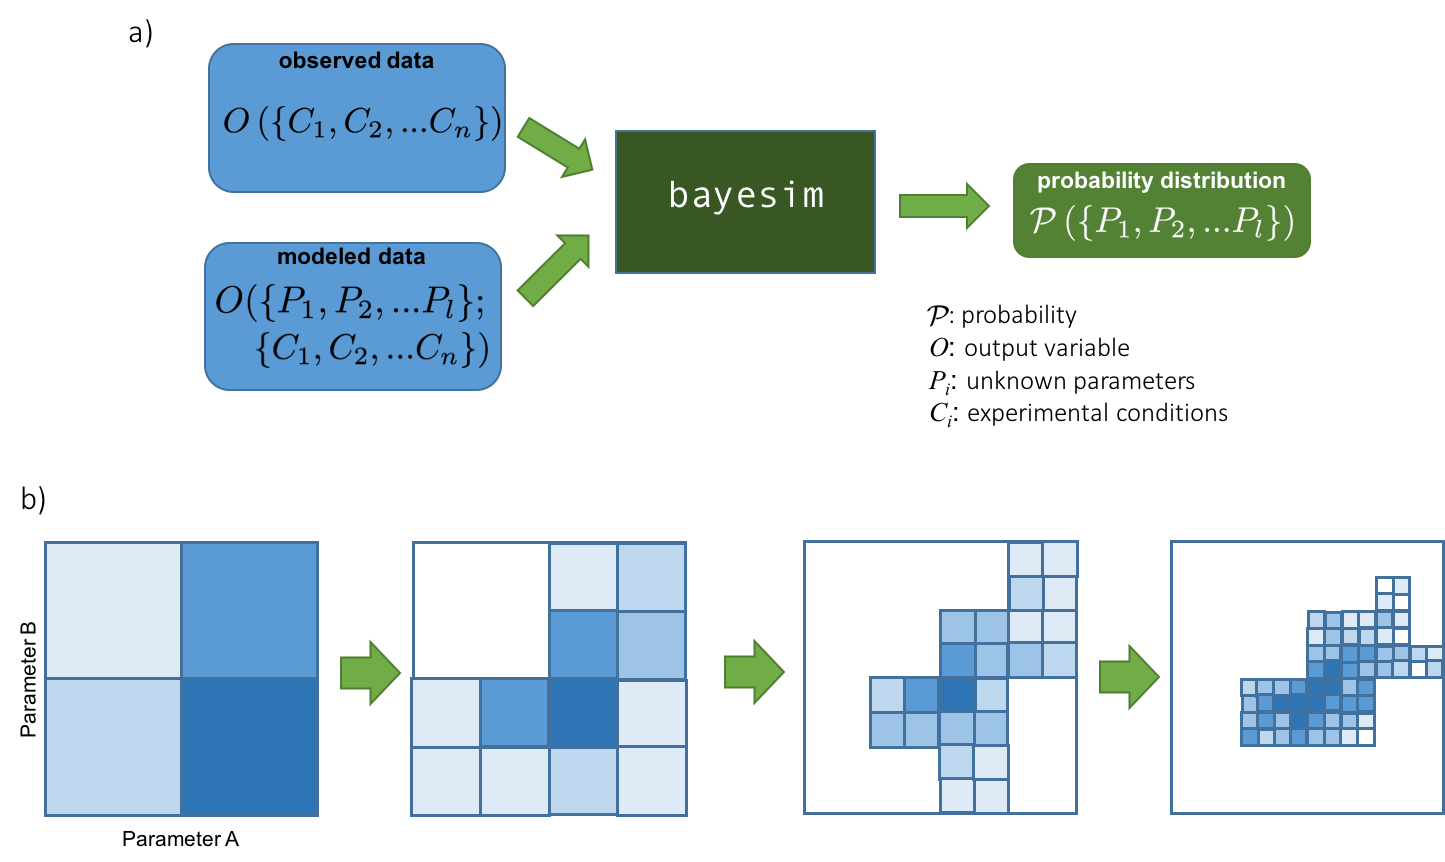
\includegraphics[width=0.7\columnwidth]{figure_1.png}
   \caption{(Figure copied from docs website for now, will make a publication-appropriate version)}
   \label{fig1}
 \end{figure}

 A high-level summary of what \texttt{bayesim} does is shown in ~\autoref{fig1}. Part (a) is a flowchart showing that observed (as a function of experimental conditions $\{C\}$ and simulated (as a function of fitting parameters $\{P\}$ and experimental conditions $\{C\}$) outputs are compared to produce a probability distribution over $\{P\}$. Part (b) schematically indicates the adaptive grid sampling approach for a hypothetical two-dimensional parameter space, wherein grid boxes exceeding some threshold probability are subdivided and lower-probability regions discarded, allowing attainment of a high fitting precision without needing to sample the entire parameter space at the same high density.

\section*{Software Architecture and Interface}

  \begin{figure}
    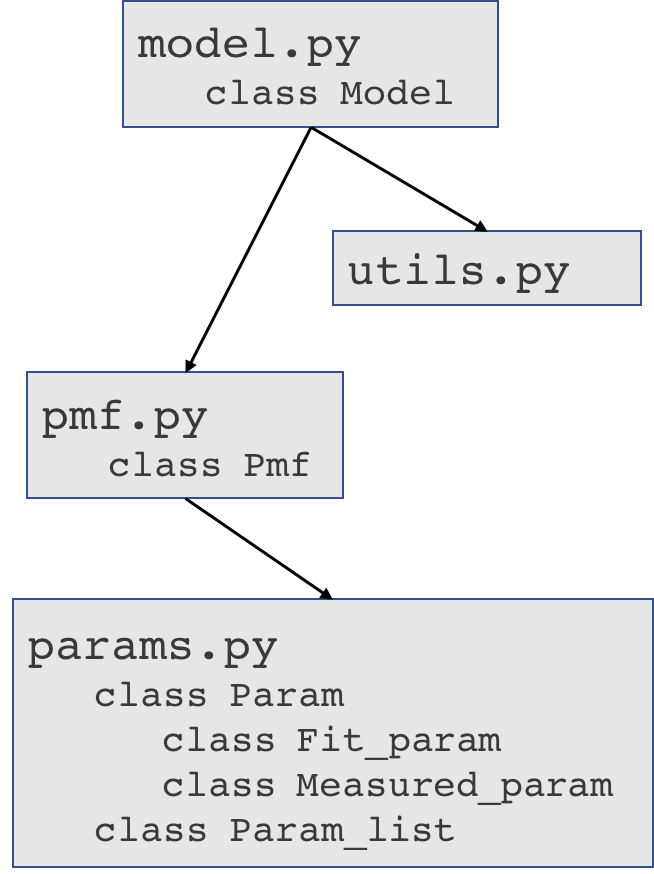
\includegraphics[width=0.55\columnwidth]{structure.png}
    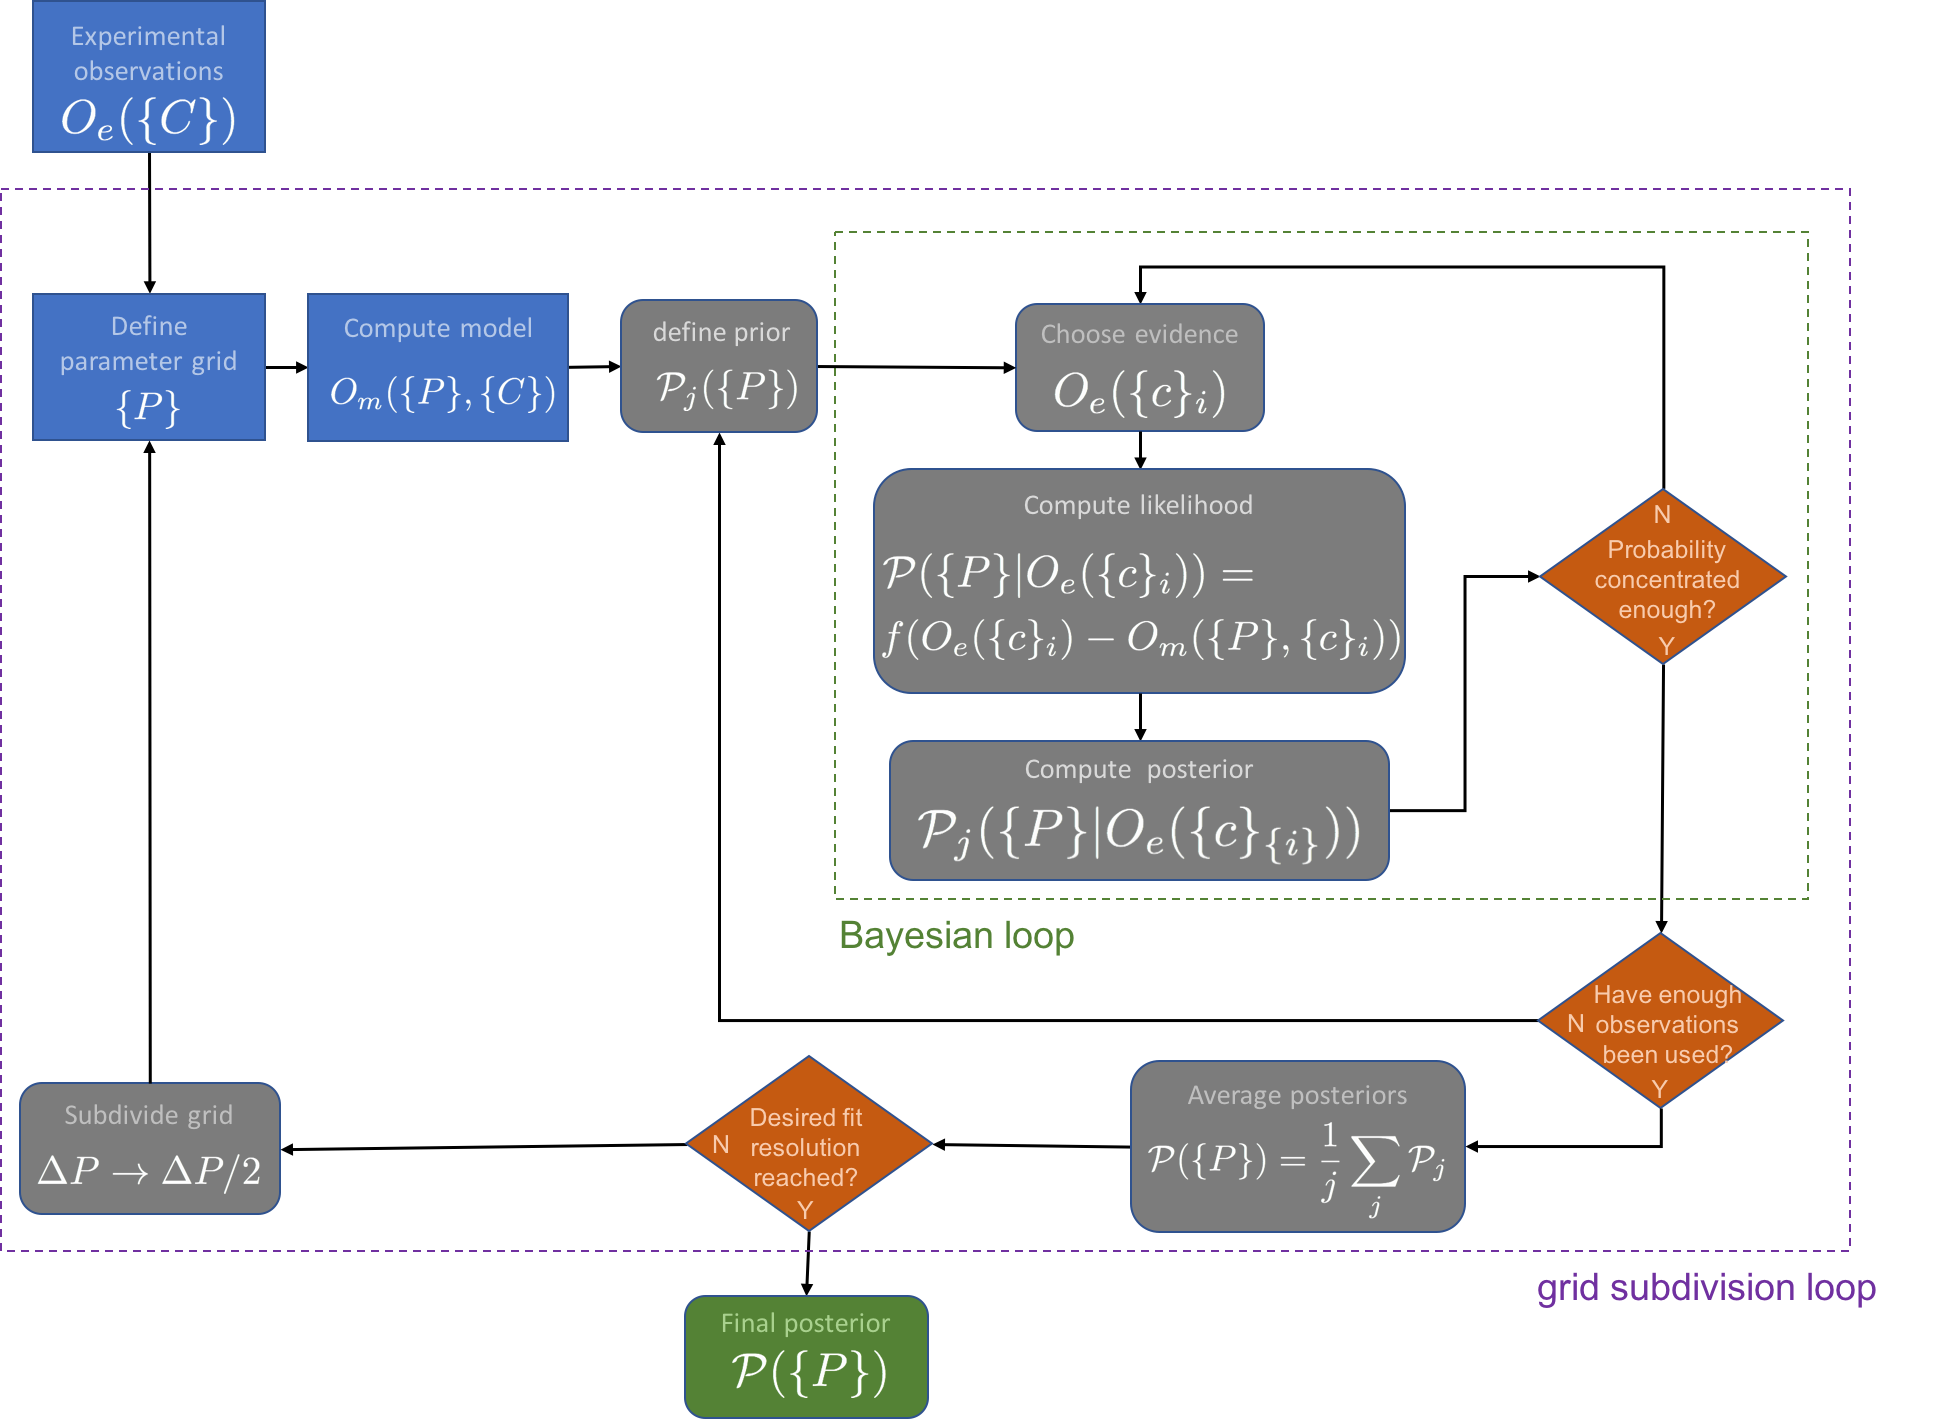
\includegraphics[width=0.4\columnwidth]{flowchart.png}
    \caption{Left: \texttt{bayesim} software structure, indicating class definitions, internal and external dependencies, and interfaces. Right: Flowchart of use of \texttt{bayesim}. (I will update these to make a more sensible figure with less white space, and also add subdivision into the loop)}
    \label{structure}
  \end{figure}

  The basic structure of \texttt{bayesim} is shown in ~\autoref{structure}a. Detailed and up-to-date documentation of classes, functions, and example applications is maintained online.~\cite{docs} The top-level object with which users interact is implemented in the \texttt{Model} class. The \texttt{params} module defines classes to store information about the various types of parameters (fitting parameters, experimental conditions, and measured output) while the \texttt{Pmf} class stores the probability distribution and implements the manipulations required for Bayesian updates.

  ~\autoref{structure}b is a flowchart of using the code, with the main inference loop surrounded by a dotted line. One first needs to provide the observed and modeled data. Observed data is accepted in HDF5 format, while modeled data can be an HDF5 file (in which case \texttt{bayesimn} will determine the fitting parameter space grid from this file), or if the fitting parameter space has been predefined, one can also attach a Python function that computes the model data (e.g. an interface to a numerical model). Observed data should have associated experimental uncertainties, or the user can indicate a fixed value of uncertainty to use for all observations upon attaching the data.

  \todo{do we need a figure for this?} Once modeled data is attached, model uncertainty can be computed. At each point in the space of experimental conditions, a matrix of the simulated output variable as a function of the fitting parameters is constructed and at each point in this matrix, the largest difference along any index is computed. This is set as the model uncertainty for this set of experimental conditions at this point in parameter space.

  At this point, the inference loop can proceed. We start with a bounded prior distribution over the entire parameter space grid and the observed data in a randomized order. We feed in one piece of evidence (i.e. one observed data point) and compute the likelihood using a Gaussian. The standard deviation for each point in the parameter space is the sum of the experimental uncertainy of that observation and the model uncertainty at that point. The posterior distribution is computed as a Bayesian update on the prior. Next, we check whether the threshold condition for concentration of probability (defined as at least some percentage (by default 90\%) of the probability mass residing in at most some percentage (by default 5\%) of the parameter space volume. If this threshold is satisfied, the current posterior is stored and the prior reset to a uniform distribution. If not, the next observation is fed in. This procedure is repeated until the requisite number (by default, 80\%) of observed data points has been used, with the final posterior being the average of every stored posterior. The posterior is calculated in this way (rather than a Bayesian multiplication through every single observed point) to avoid numerical errors that can arise if very small numbers are multiplied together.

  Now the grid can be subdivided. The user defines a threshold probability (by default 0.001) for a grid box to possess, and all boxes with greater than this probability, as well as all their immediate neighbors, are divided in two along every parameter. \texttt{bayesim} saves a list of the new model calculations that need to be done for inference to proceed again, and the user provides these, again either as a callable or an HDF5 file. For the next round of inference, the user can also define a ``bias" parameter from 0 to 0.5 (default 0) that will mix in some fraction of the posterior from the previous step with the uniform distribution over this new grid.

  This overall procedure can be repeated as many times as the user wishes to get a more precise fit -- eventually, the concentration of probability becomes limited by experimental rather than model uncertainty. There is also an option to define a minimum width for a box along any parameter direction, and if a box is already less than this width, \texttt{bayesim} will not subdivide in that direction.

  The most flexible way to interact with \texttt{bayesim} is via Python scripting or through literate programming in a Jupyter notebook. There is also a command line interface (CLI) for users less familiar with coding in Python.

  \texttt{bayesim} relies on a variety of external open-source packages. These include \texttt{numpy}~\cite{numpy} and \texttt{scipy}~\cite{scipy} for a variety of mathematical functions and vectorized implementations, \texttt{joblib}~\cite{joblib} for simple parallelism, \texttt{deepdish}~\cite{deepdish} for saving and loading HDF5 files, \texttt{pandas}~\cite{pandas} for data manipulation, and \texttt{matplotlib}~\cite{mpl} for visualization.

\section*{Application Examples}
  \subsection{Ideal Diode Model}
    As a first example, we fit a simple two-parameter model of solar cell current density $J$ (as a function of voltage $V$ and temperature $T$) known as the ideal diode model:

    \begin{equation}
      J(V,T) = J_L+J_0\left(\exp{\frac{qV}{nkT}}-1\right)
      \label{ID_eqn}
    \end{equation}

    where $k=8.61733\times 10^{-5}$ eV/K is Boltzmann's constant, by convention $J_L$ (the light current) is negative and $J_0$ (the saturation current) is positive but strongly dependent on temperature, a dependence we can approximate as:

    \begin{equation}
      J_0 \approx B'T^{3/n}\exp{\left(\frac{-E_{g0}}{nkT}\right)}
    \end{equation}

    where $E_{g0}$ is the zero-temperature bandgap of the material. For this example, we will set this to 1.2 eV and $J_L$ to -0.03 mA/cm$^2$. There are thus two parameters to be fit, the coefficient $B'$ (which can range over a wide variety of values) and the ideality factor $n$ (which is by definition between 1 and 2).

    \begin{figure}
      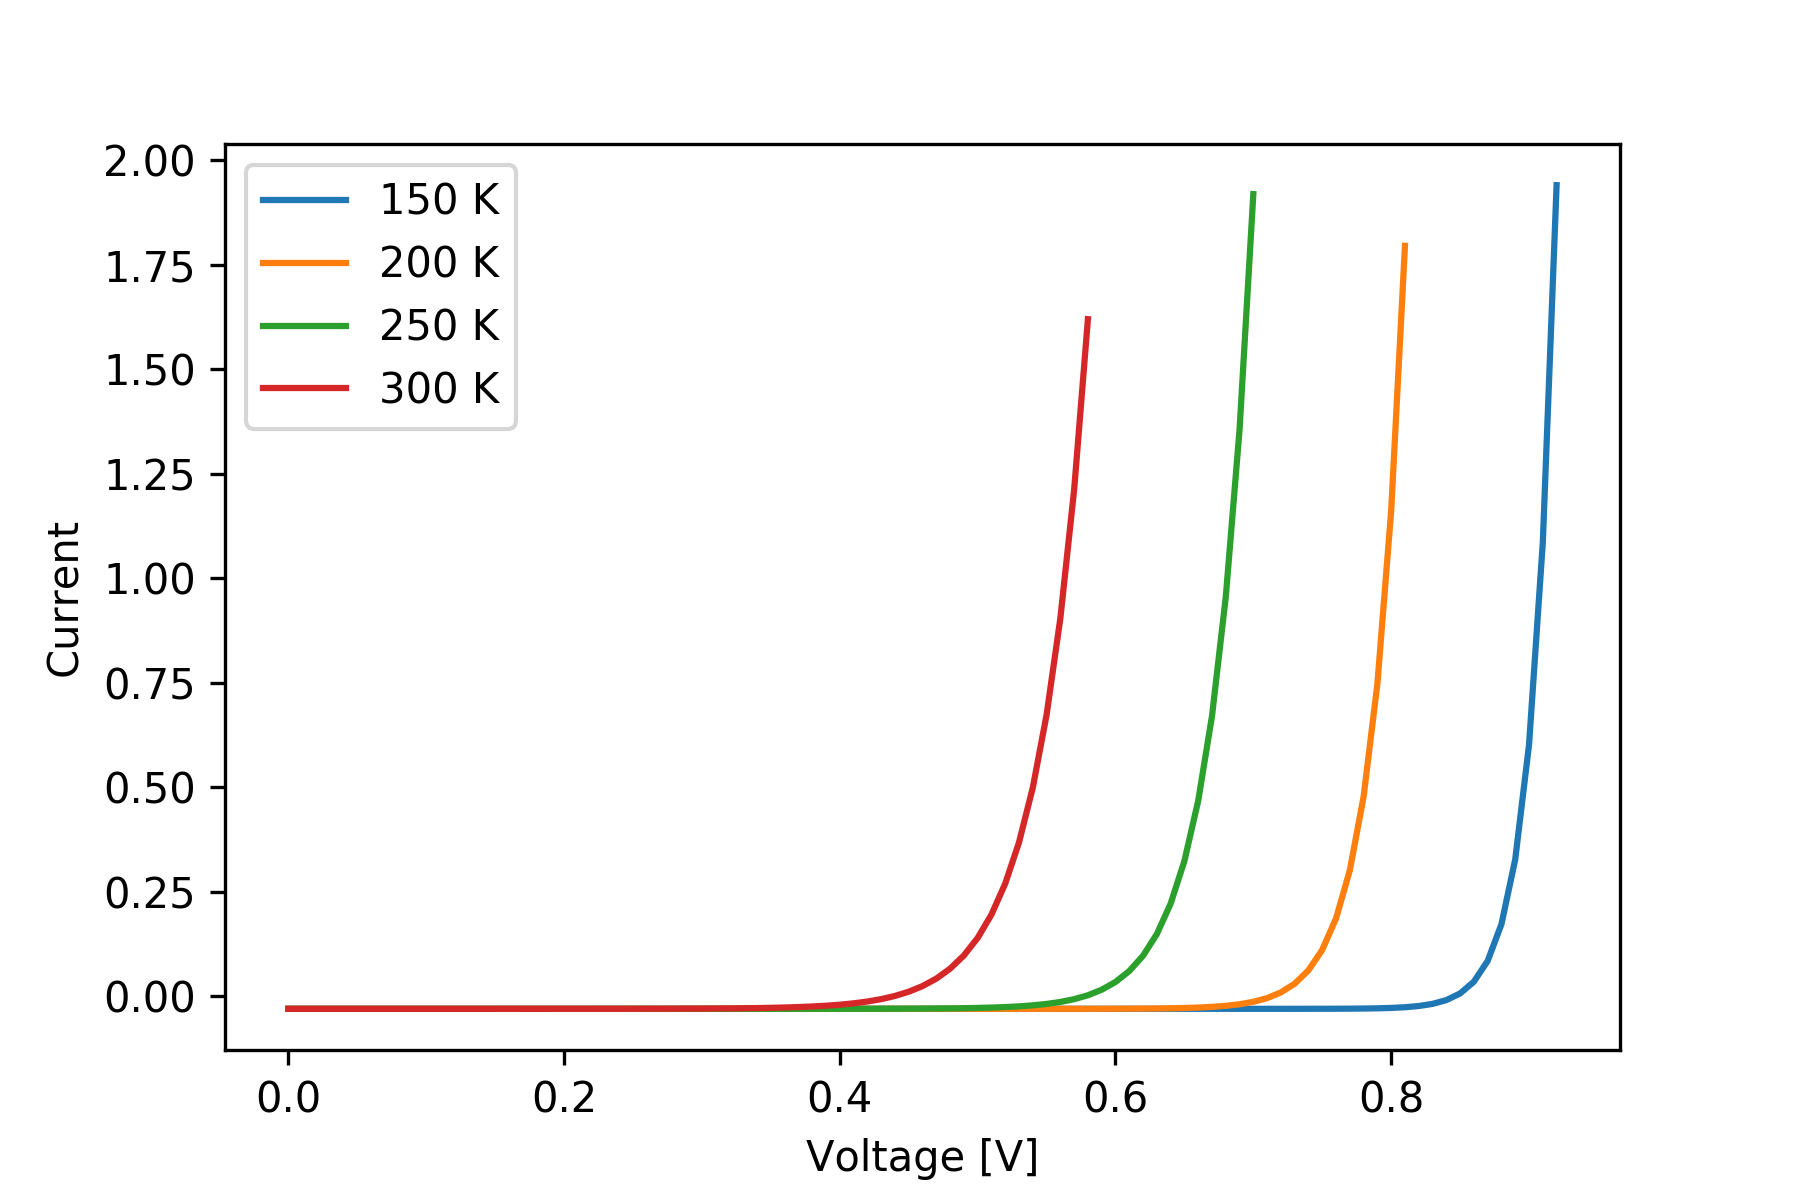
\includegraphics[width=0.45\columnwidth]{diode_obs.png}
      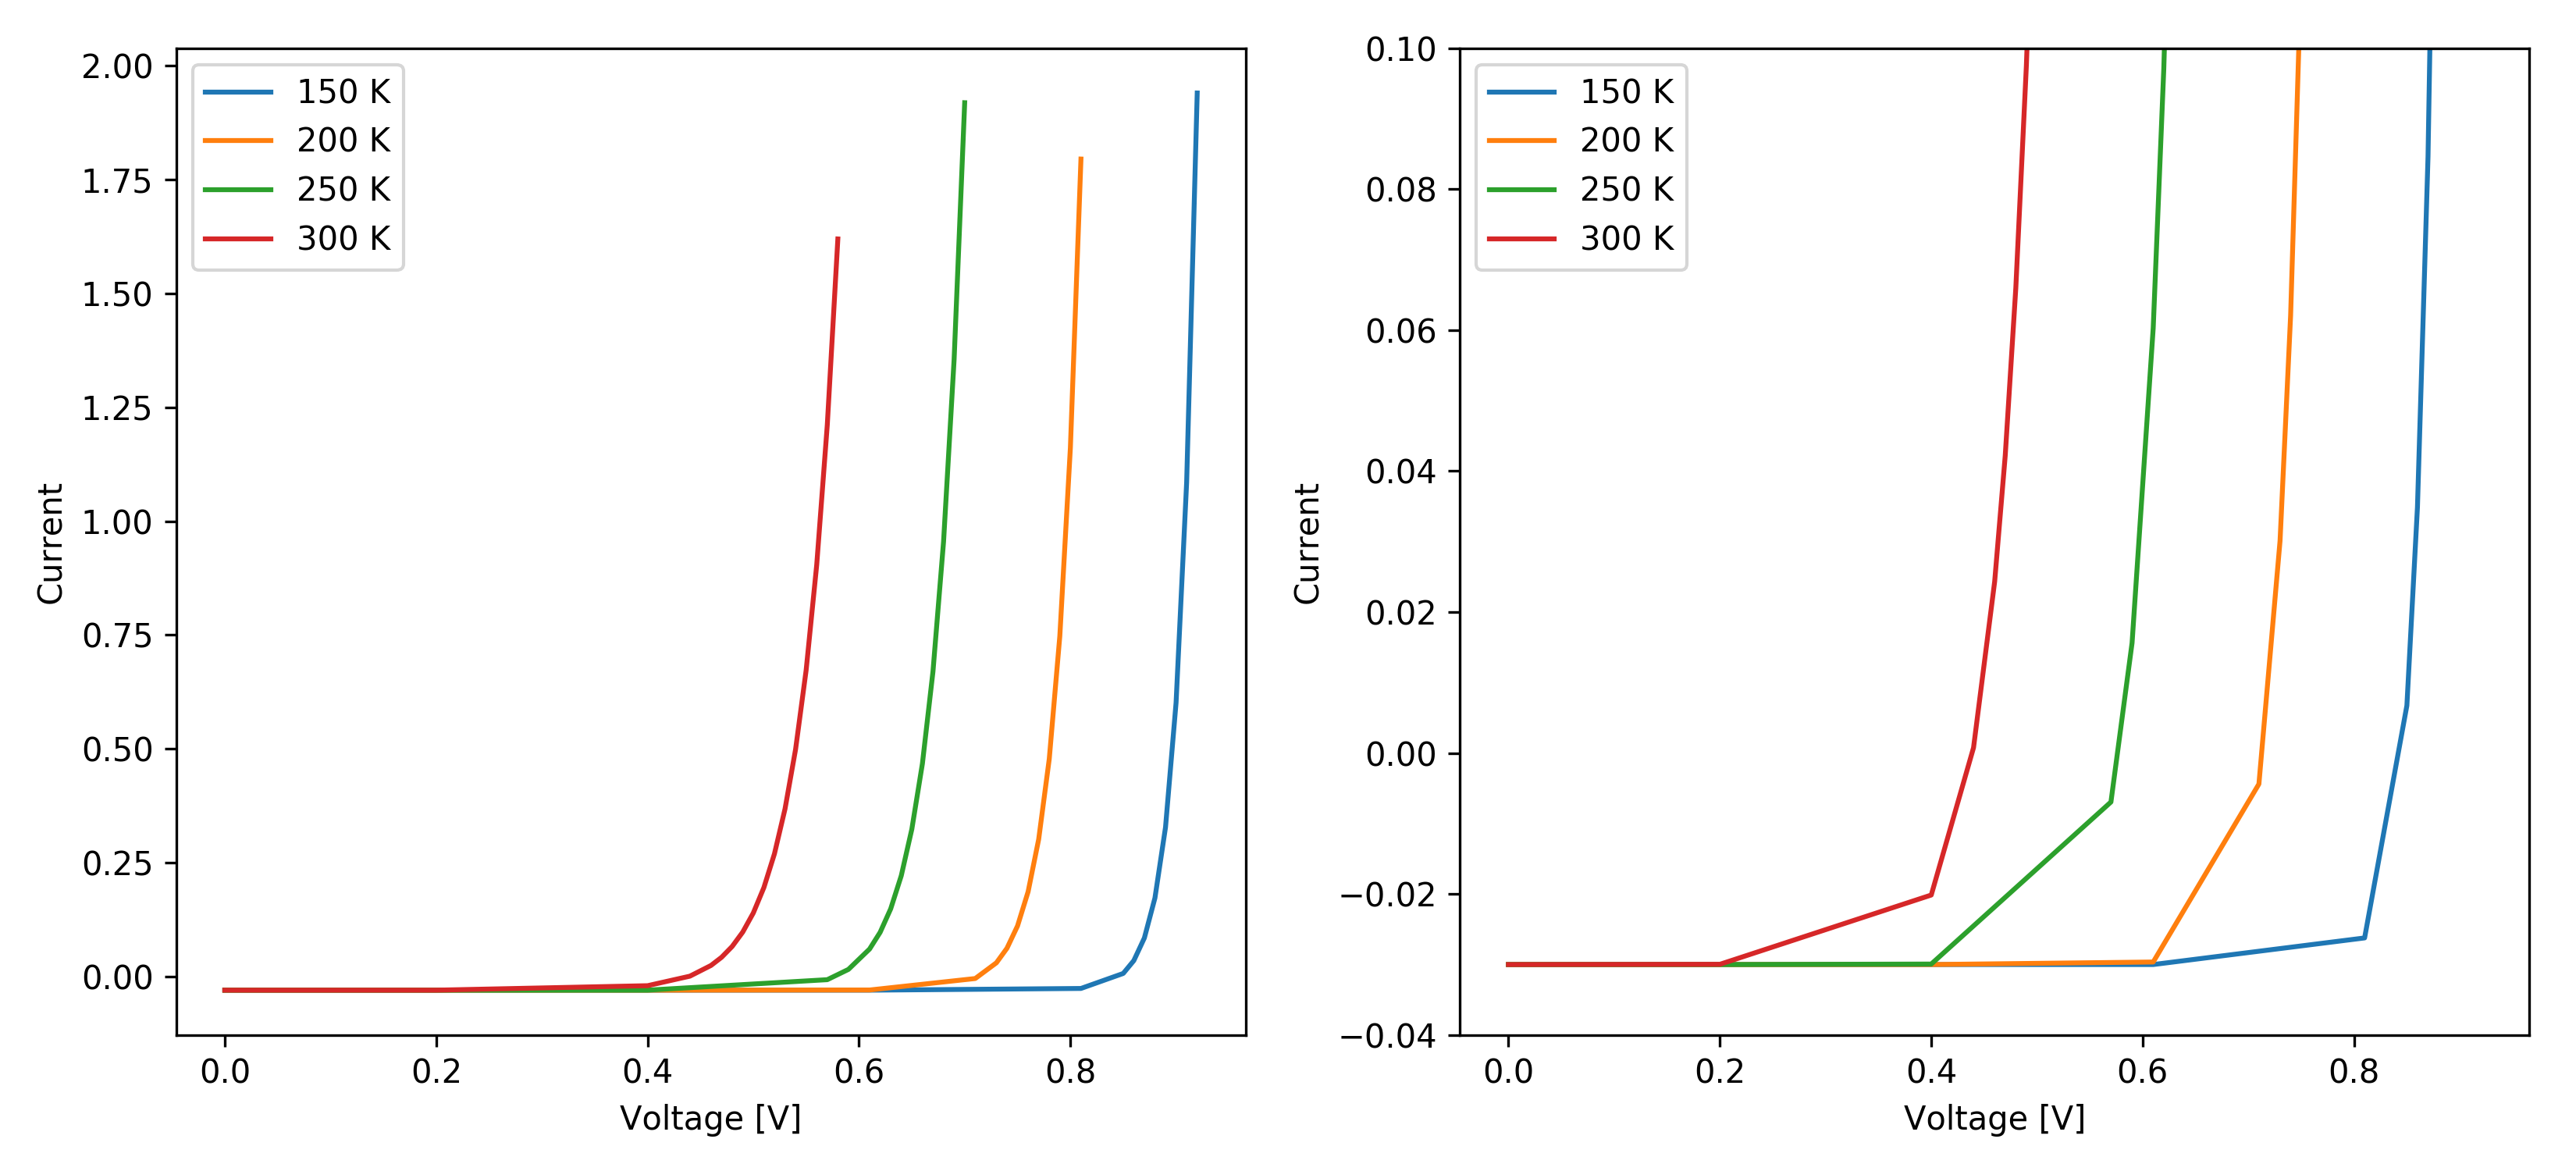
\includegraphics[width=0.45\columnwidth]{diode_obs_zoom.png}
      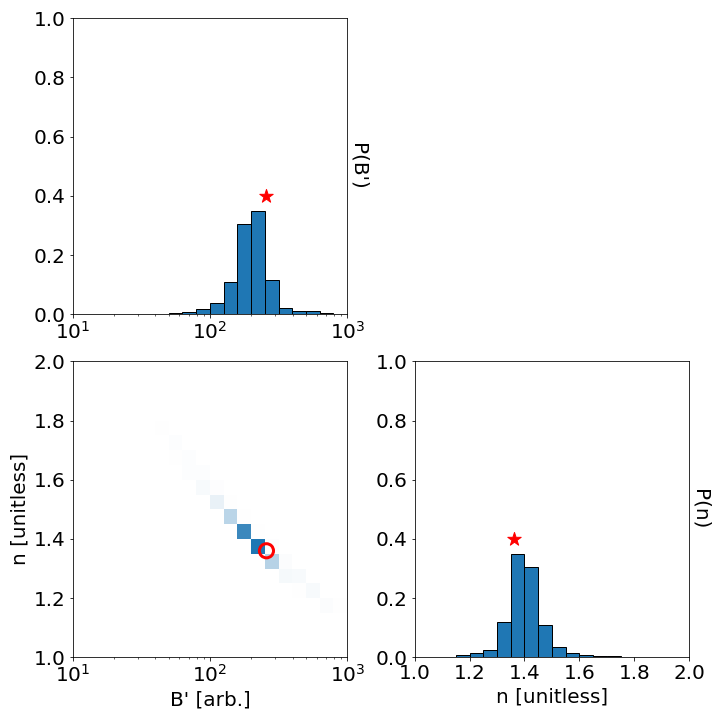
\includegraphics[width=0.3\columnwidth]{diode_pmf_1.png}
      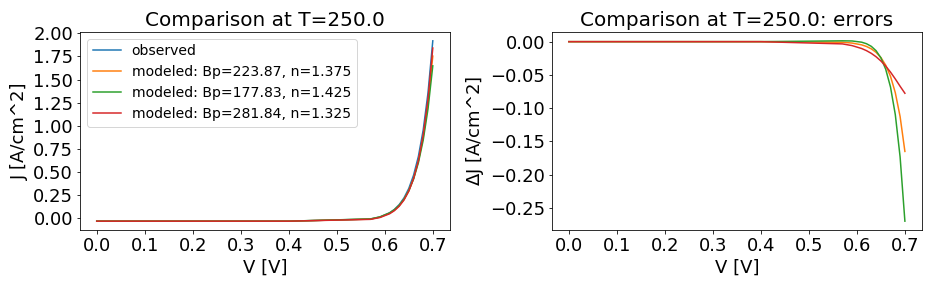
\includegraphics[width=0.65\columnwidth]{diode_comp_1.png}
      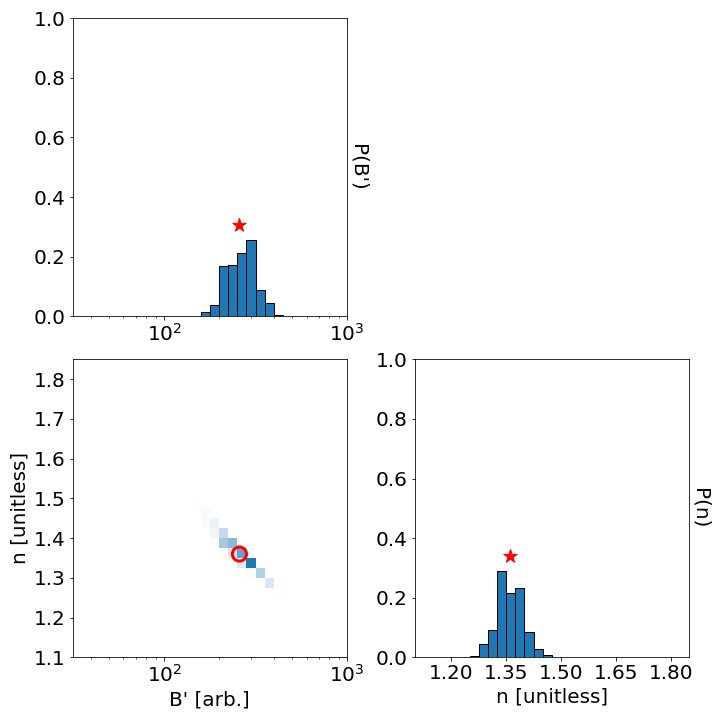
\includegraphics[width=0.3\columnwidth]{diode_pmf_2.png}
      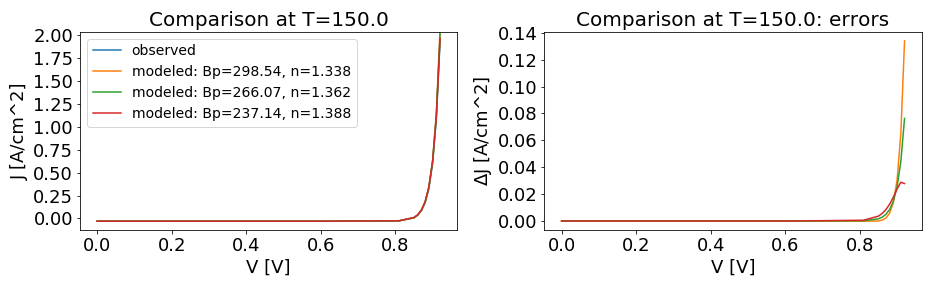
\includegraphics[width=0.65\columnwidth]{diode_comp_2.png}
      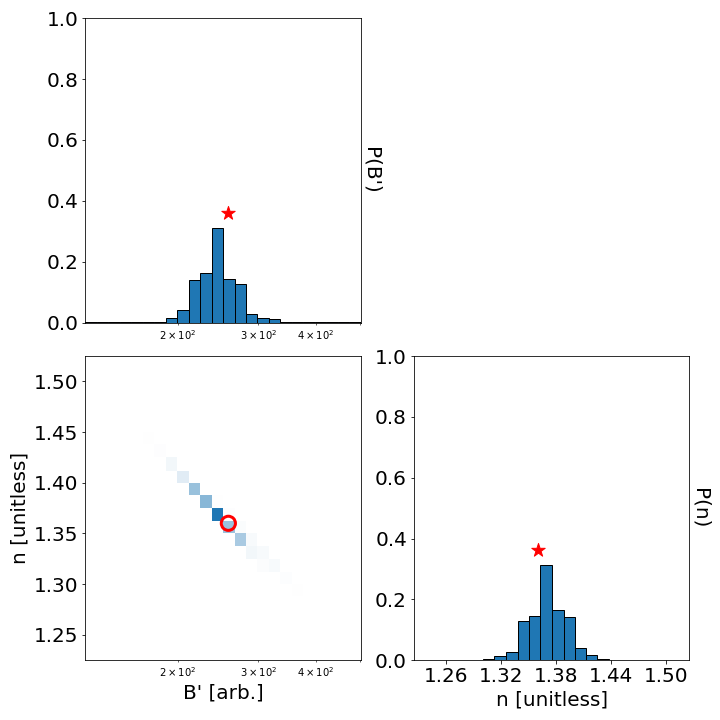
\includegraphics[width=0.3\columnwidth]{diode_pmf_3.png}
      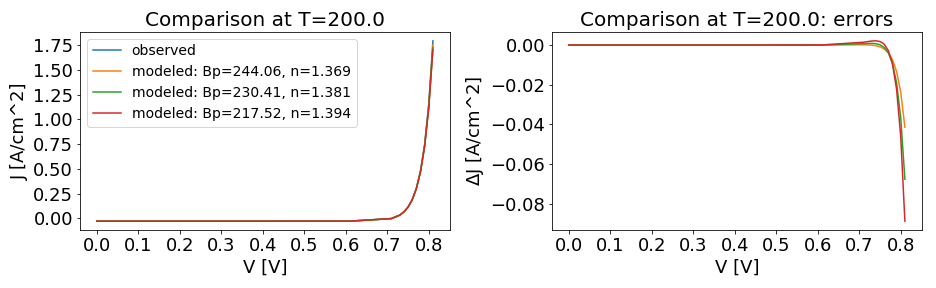
\includegraphics[width=0.65\columnwidth]{diode_comp_3.png}
      \caption{a) ``Observations" generated by ideal diode model, Equation~\ref{ID_eqn}, b) Observed data saved by \texttt{bayesim}, with zoom to show where neglected data points were, Next three rows: PMF's, comparisons of highest three probability model points with observed data, and absolute errors thereof, on the initial grid, and after one and two subdivisions, respectively. ``True'' values for the parameters indicated on the PMF in red. (this figure is a giant data dump right now; I'm figuring out how to make it less terrifyingly overwhelming - like possibly overlaying all three PMF's onto one plot in different colors)}
      \label{ID_data}
    \end{figure}

    As validation, we generate the ``observations" using the same model we'll use for fitting, with parameter values of $n=1.36$ and $B'=258$, and four temperature values of 150, 200, 250, and 300 K. These ``observations" are shown in ~\autoref{ID_data}a. When \texttt{bayesim} imports observed data, it can optionally discard data points that are very close by to each other in order to reduce computational load on modeling less informative points - this capacity is demonsrated in ~\autoref{ID_data}b.

    The next three rows of ~\autoref{ID_data} show the posterior distributions, comparison of JV data between observations and the three highest-probability model points, and absolute errors thereof, on the initial grid and after one and two rounds of subdivision. Note that the ranges on the parameter values get narrower as does the scale of absolute errors.

  \subsection{SnS Solar Cell}
    \begin{itemize}
      \item more practical example - replicating fit from Joule paper
      \item figure 4 showing PMF and comparison of JV curves
    \end{itemize}


\section*{Conclusions}
 talk about broader applicability of approach

\section*{Acknowledgements}

\section*{Appendix}
 \begin{itemize}
   \item include minimal code to run ideal diode example
   \item link to Github repo (which has installation instructions and documentation as well as list of planned future features)
  \end{itemize}

\bibliography{biblio}
\bibliographystyle{ieeetr}

\end{document}
